\documentclass[12pt]{beamer}

\usepackage{color}
\usepackage[normalem]{ulem}

% Esto es para que el LaTeX sepa que el texto est� en espa�ol:
\usepackage[spanish]{babel}

% Include figure files.
\usepackage{graphicx}

% Author, Title, etc.

\title[Bases de Datos Espaciales] 
{%
  Bases de Datos Espaciales%
}

\author[Del Piano]
{
  Nicol\'as Del Piano
}

\date
{
Bases de Datos Avanzadas
}

\mode<presentation>{
\usetheme{boxes}
\useinnertheme{}
\usecolortheme{whale}
}
\setbeamercolor{structure}{fg=blue!50!black!70}
\setbeamertemplate{footline}[frame number]
\setbeamerfont{page number in head/foot}{size=\normalsize}

\newenvironment{variableblock}[3]{%
  \setbeamercolor{block body}{#2}
  \setbeamercolor{block title}{#3}
  \begin{block}{#1}}{\end{block}}

\setbeamercolor{block title}{bg=red!60,fg=black}
%\setbeamertemplate{blocks}[rounded][shadow=true] 
\setbeamercolor{postit}{bg=yellow!50!white}
\setbeamercolor{bluelick}{bg=blue!50!white}

\begin{document}
\frame{\titlepage}
\begin{frame}
\frametitle{Recorrido}
\begin{itemize}
\item Pensando Espacialmente
\item Bases de Datos Espaciales
\begin{enumerate}
\item Definici\'on
\item DBMS
\end{enumerate}
\item Hacia un Modelo de Datos Espacial
\begin{enumerate}
\item Objetos en el espacio
\item Espacio
\item Organizando el espacio
\item Tipos de Datos y \'Algebras Espaciales
\item Consultas
\end{enumerate}
\item Indexaci\'on Espacial
\begin{enumerate}
\item R-Tree
\item Estructuras
\end{enumerate}
\item Estado del Arte
\end{itemize}
\end{frame}
\begin{frame}
\frametitle{Pensar Espacialmente}
?`D\'onde est\'a esto? ?`Cu\'anto tardo para llegar?\\
\ \\
Hoy en d\'ia tenemos grandes herramientas para responder este tipo de preguntas.\\
\ \\
Google Maps, Virtual Earth, MapQuest, Yahoo, etc...
%\begin{variableblock}{Definici\'on}{bg=blue!50!white!70,fg=white}{bg=blue!50!black!70,fg=white}
%\textit{Hola mam\'a}
%\end{variableblock}
\end{frame}

\begin{frame}
\frametitle{Pensar Espacialmente}
Yendo m\'as all\'a, las organizaciones han descubierto que estas herramientas son un gran recurso para analizar patrones de datos.\\
\ \\
Por ejemplo, una popular empresa de pizzas, trazando los recorridos de las direcciones de los "pizza lovers", puede encontrar facilmente d\'onde inaugurar su nuevo local.
\end{frame}

\begin{frame}
\frametitle{Pensar Espacialmente, ?`en un DBMS relacional?}
La informaci\'on es almacenada y controlada en los DBMS relacionales.\\
\ \\
Si bien son muy populares y responden a la mayor\'ia de las consultas, la visi\'on real es que muchas de ellas son incapaces de manejar datos espaciales, o son poco amigables.\\
\ \\
?`Por qu\'e?\\
\ \\
El rol tradicional de un DBMS es y ha sido almacenar informaci\'on relacionada al mundo de los negocios.
\end{frame}


\begin{frame}
\frametitle{Pensar Espacialmente, ?`en un DBMS relacional?}
Los datos que residen en esas grandes bases de datos es simple (nombres, saldos, direcciones, etc\'etera).\\
\ \\
Por ejemplo, una consulta como "listar todos los empleados cuyo sueldo es mayor a X" puede ser simple y eficientemente respondida, a\'un en bases de datos gigantes.\\
\ \\
Pero, ?`qu\'e sucede si quiero saber: "listar todos los empleados que residan a menos de 10 km de la compan\'ia"?\\
\ \\
En los DBMS relacionales, es posible contestar estas preguntas... pero es totalmente \textbf{ineficiente}.
\end{frame}


\begin{frame}
\frametitle{Pensar Espacialmente}
En conclusi\'on, en muchas \'areas existe la necesidad de administrar informaci\'on \textit{geom\'etrica}, \textit{geogr\'afica} o \textit{espacial}, es decir, informaci\'on relacionada con el \textbf{espacio}.\\
\ \\
Las \textbf{Bases de Datos Espaciales} pueden ayudarnos.
\end{frame}

\begin{frame}
\frametitle{Aplicaciones}
Sistemas de Informaci\'on Geogr\'afica.\\
\ \\
Bases de Datos Multimedia.\\
\ \\
Im\'agenes satelitales.\\
\ \\
Modelo de circuitos integrados de gran tama\~no.\\
\ \\
Censos.\\
\ \\
Ciencias Ambientales.\\
\ \\
Astronom\'ia.
\end{frame}

\begin{frame}
\frametitle{?`Qui\'en se beneficia?}
\underline{Usuario de celular}: ?`D\'onde est\'a la siguiente estaci\'on de servicio? ?`Hay una camino a casa?\\
\ \\
\underline{M\'edico}: Basado en el siguiente MRI, ?`hemos tratado a alguien con el mismo resultado?\\
\ \\
\underline{Bi\'ologo molecular}: ?`Est\'a la topolog\'ia de la bios\'intesis del gel amino\'acido en el genoma descubierto 	en otra secuencia de la base de datos?\\
\ \\
\underline{Astr\'onomo}: Buscar todas las galaxias dentro de dos minutos de arcos de qu\'asares.\\
\ \\
\underline{Climat\'ologo}: Testear y verificar mi nuevo modelo clim\'atico. 
\end{frame}

\begin{frame}
\frametitle{?`Qu\'e se busca?}
Tener soporte para representar este tipo de tablas:\\
\begin{center}
\begin{tabular}{|c|c|c|}
\hline
Id & Pa\'is & Geograf\'ia \\
\hline
1 & Argentina & 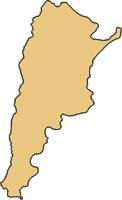
\includegraphics[width=0.6cm,height=1.2cm]{Imagenes/argentina.jpg}\\
\hline
2 & Brasil & 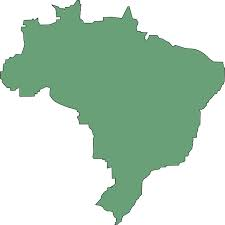
\includegraphics[width=1.5cm,height=1.5cm]{Imagenes/brasil.jpg}\\
\hline
\end{tabular}\\
\end{center}
\ \\
Y adem\'as brindar herramientas que permitan comparar eficientemente datos como los de la tercer columna.


\end{frame}

\begin{frame}
\frametitle{Bases de Datos Espaciales}
\begin{variableblock}{Definici\'on$_{1}$}{bg=blue!50!white!70,fg=white}{bg=blue!50!black!70,fg=white}
\textit{Es una base de datos que es optimizada para almacenar y consultar informaci\'on relacionada a objetos en el espacio, incluyendo puntos, l\'ineas y pol\'igonos.}
\end{variableblock}

\begin{variableblock}{Definici\'on$_{2}$}{bg=blue!50!white!70,fg=white}{bg=blue!50!black!70,fg=white}
\textit{Es una colecci\'on de datos espaciales y no espaciales que est\'an interrelacionados.}
\end{variableblock}


\end{frame}

\begin{frame}
\frametitle{Bases de Datos Espaciales}
Deben permitir la descripci\'on de los objetos espaciales mediante tres caracter\'isticas:\\
\ \\
\begin{itemize}
\item \textbf{Atributos}: qu\'e es un objeto de acuerdo a sus caracter\'isticas.
\item \textbf{Localizaci\'on}: conocer d\'onde est\'a el objeto y qu\'e lugar ocupa.
\item \textbf{Topolog\'ia}: mejorar la interpretaci\'on sem\'antica del contexto y establecer jerarqu\'ias.
\end{itemize}
\end{frame}

\begin{frame}
\frametitle{DBMS Espacial}
\begin{variableblock}{Definici\'on}{bg=blue!50!white!70,fg=white}{bg=blue!50!black!70,fg=white}
\begin{itemize}
\item \textit{Un SDBMS es un DBMS.}
\item \textit{Ofrece datos espaciales (SDTs) en su modelo de datos y su lenguaje de consulta.}
\item \textit{Soporta tipos de datos espaciales en su implementaci\'on, proveyendo al menos indexaci\'on espacial y algoritmos eficientes para joins espaciales.}
\end{itemize}
\end{variableblock}
\end{frame}

\begin{frame}
\frametitle{DBMS Espacial}
Un SDBMS es un DBMS.\\
\ \\
Suena trivial; refleja el hecho de que la informaci\'on espacial o geom\'etrica est\'a, en pr\'actica, conectada con la informaci\'on "no-espacial".\\
\ \\
El SDBMS tiene propiedades adicionales para manejar datos espaciales. 
\end{frame}

\begin{frame}
\frametitle{DBMS Espacial}
Tipos de datos espaciales.\\
\ \\
POINT, LINE, REGION, etc\'etera.\\
\ \\
Proveen una abstracci\'on fundamental para modelar la estructura de entidades geom\'etricas en el espacio, as\'i como sus relaciones, propiedades y operaciones.
\end{frame}

\begin{frame}
\frametitle{Objetivos de un SDBMS}
Integrar la representaci\'on y manipulaci\'on de datos geom\'etricos y espaciales con los datos no espaciales en un nivel l\'ogico.\\
\ \\
Proveer un soporte eficiente para almacenar y procesar datos a nivel f\'isico.
\end{frame}

\begin{frame}
\frametitle{Requerimientos de un SDBMS}
El lenguaje de consulta debe incorporar nuevas funciones sobre componentes geom\'etricos.\\
\ \\
Utilizar m\'etodos de acceso eficientes.\\
\ \\
Incorporar nuevos algoritmos para procesar consultas que satisfacen combinaciones de restricciones.\\
\ \\
La representaci\'on l\'ogica debe ser extendida a datos geom\'etricos.\\
\ \\
Capacidad de manejar grandes colecciones de objetos geom\'etricos.
\end{frame}

\begin{frame}
\begin{center}\textbf{HACIA UN MODELO ESPACIAL}
\end{center}
\end{frame}

\begin{frame}
\frametitle{Modelando Datos Espaciales}
Asumiendo aplicaciones 2-d y GIS, existen dos aspectos importantes que necesitan ser representados:\\
\ \\
\begin{itemize}
\item \textbf{Objetos en el Espacio}: distinguir entre entidades espaciales de acuerdo a su representaci\'on geom\'etrica.
\item \textbf{Espacio}: describir cada punto del espacio, es decir, tener una idea de la representaci\'on del espacio mismo.
\end{itemize}
\end{frame}

\begin{frame}
\frametitle{Modelando Datos Espaciales}
Los datos espaciales tienen las siguientes desventajas:
\begin{itemize}
\item Estructura compleja.
\item Las SBD tienden a ser muy grandes.
\item No existe un \'algebra est\'andar.
\item Operadores no cerrados.
\item Costo computacional elevado.
\end{itemize}
Es por ello que hay que implementar algoritmos y estructuras de datos que optimicen la manipulaci\'on de los mismos.
\end{frame}

%\begin{frame}
%\frametitle{Holis}
%\end{frame}

\begin{frame}
\frametitle{Objetos en el Espacio}
Objetos \'unicos e individuales.\\
\ \\
Para modelarlos, las abstracciones fundamentales son el \textit{punto}, la \textit{l\'inea} y la \textit{regi\'on} (pol\'igono).\\
\ \\
\begin{center}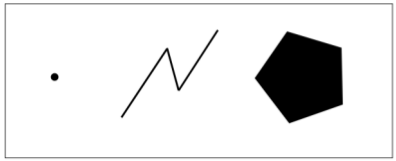
\includegraphics[width=8cm,height=3cm]{Imagenes/figurasgeom.png}
\end{center}

\end{frame}

\begin{frame}
\frametitle{Punto}
Un punto representa el aspecto geom\'etrico de un objeto para el cual lo \'unico relevante es su localizaci\'on en el espacio.\\
\ \\
Por ejemplo, una ciudad puede ser modelada como un punto en un mapa.\\
\ \\
\begin{center}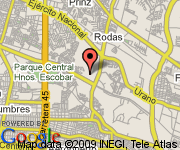
\includegraphics[width=3cm,height=3cm]{Imagenes/mapa1.png}
\end{center}
\end{frame}

\begin{frame}
\frametitle{L\'inea}
Una l\'inea representa es la abstracci\'on b\'asica del movimiento a trav\'es del espacio, o conexiones en espacio.\\
\ \\
Por ejemplo, r\'ios, carreteras, cables de tel\'efono, etc\'etera.\\
\ \\
Usualmente representadas como \textit{polil\'ineas}, i.e, secuencias de segmentos.
\end{frame}

\begin{frame}
\frametitle{Regi\'on o pol\'igono}
Una regi\'on es una abstracci\'on para algo que tenga una extensi\'on en el espacio 2-d.\\
\ \\
Por ejemplo un pa\'is, un lago, un parque nacional, etc\'etera.\\
\ \\
Una regi\'on puede tener huecos y puede ser conformada por distintos objetos del espacio.\\
\ \\
\begin{center}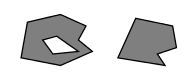
\includegraphics[width=4cm,height=1.8cm]{Imagenes/poligonos.png}
\end{center}
\end{frame}

\begin{frame}
\frametitle{Espacio}
Hay que caracterizar los puntos del espacio.\\
\ \\
De esta forma, podemos modelar mapas tem\'aticos que indiquen por ejemplo, la divisi\'on de un pa\'is en provincias.\\
\ \\
Existen dos importantes instancias en las colecciones de objetos relacionadas espacialmente (espacio).\\
\ \\
Son las \textit{particiones} y las \textit{redes}.\\
\end{frame}

\begin{frame}
\frametitle{Particiones}
Una partici\'on puede ser vista como un conjunto de regiones que son disjuntas.\\
\ \\
La adyacencia en este caso tiene un inter\'es particular; pares de regiones que tienen frontera com\'un.\\
\ \\
Pueden ser usadas para representar mapas.
\ \\
\begin{center}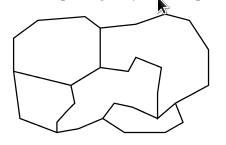
\includegraphics[width=3cm,height=1.8cm]{Imagenes/particion.png}
\end{center}
\end{frame}

\begin{frame}
\frametitle{Redes}
Una red puede ser vista como un grafo embebido en el plano.\\
\ \\
Est\'a compuesta por un conjunto de objetos puntos (nodos) y un conjunto de objetos l\'ineas (aristas).\\
\ \\
Pueden ser usadas para representar elementos geogr\'aficos como carreteras, r\'ios, transportes p\'ublicos, etc\'etera.
\ \\
\begin{center}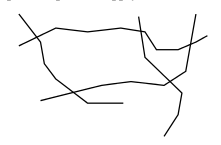
\includegraphics[width=3cm,height=1.8cm]{Imagenes/red.png}
\end{center}
\end{frame}

\begin{frame}
\frametitle{Otras abstracciones}
Hemos mencionado hasta aqu\'i las m\'as comunes.\\
\ \\
Obviamente, existen otras como las \textit{particiones anidadas} (e.g. un pa\'is divido en provincias, y a su vez cada provincia en estados), o los modelos de terrenos digitales, para representar relieves.\\
\ \\
\begin{center}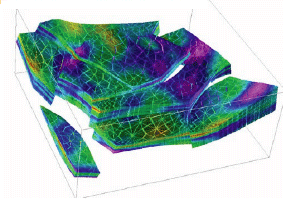
\includegraphics[width=3cm,height=2.5cm]{Imagenes/relieves.png}
\end{center}
\end{frame}

\begin{frame}
\frametitle{Organizando el Espacio}
La geometr\'ia Euclidiana no es adecuada como una base para modelar en las bases de datos espaciales.\\
\begin{itemize}
\begin{small}
\item El espacio Eucl\'ideo es \textbf{cont\'inuo}, i.e., los puntos son representados como un par de n\'umeros reales: $p = (x,y) \in \mathbf{R}^{2}$.
\item Pero la computadora trabaja en forma \textbf{discreta}.
\begin{itemize}
\item $\Rightarrow$ el espacio es representado por un \textit{raster discreto}.
\end{itemize}
\end{small}
\end{itemize}
\textbf{Ejemplo:} Intersecci\'on de dos l\'ineas
\begin{itemize}
\begin{small}
\item El punto de intersecci\'on es redondeado al punto de la grilla m\'as cercano.
\item Una prueba para determinar si el punto de intersecci\'on est\'a en una de las l\'ineas determina un resultado falso.
\end{small}
\end{itemize}
\begin{center}
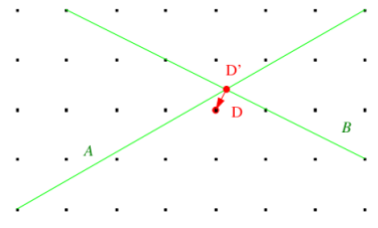
\includegraphics[width=4cm,height=3cm]{Imagenes/1.png}
\end{center}

\end{frame}

\begin{frame}
\frametitle{Organizando el Espacio}
\textbf{Soluci\'on:} Definir una base geom\'etrica discreta para modelar el espacio, as\'i tambi\'en como para lidiar con su implementaci\'on.\\
\ \\
Dos intentos para una base geom\'etrica:\\
\begin{itemize}
\item \textbf{Simplicial complexes} (Frank \& Kuhn)
\item \textbf{Realms} (G\"uting \& Schneider)
\end{itemize}
\end{frame}

\begin{frame}
\frametitle{Organizando el Espacio: Simplicial Complexes}
Conceptos b\'asicos de \textbf{simplicial complexes}
\begin{itemize}
\item \textbf{d-simplex}: Un objeto de dimensi\'on d
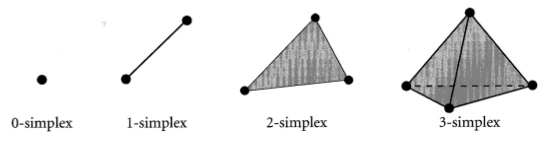
\includegraphics[width=6cm,height=2cm]{Imagenes/2.png}
\item \textbf{Simplicial Complex:} Un conjunto finito de simplices tales que la intersecci\'on de dos simplices cualquiera en el conjunto es un componente usado en los simplices.
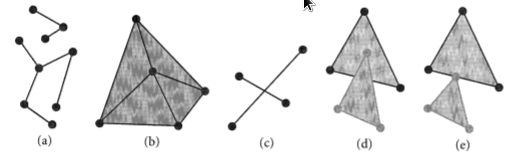
\includegraphics[width=6cm,height=2cm]{Imagenes/3.png}
\end{itemize}
\end{frame}

\begin{frame}
\frametitle{Organizando el Espacio: Realm}
\textbf{Realm:} Un conjunto finito de puntos y segmentos de l\'ineas definidos sobre una grilla tal que:
\begin{small}
\begin{itemize}
\item cada punto o punto final de los segmentos es un punto en la grilla
\item cada punto final de un segmento es un punto del realm
\item ning\'un punto del realm se encuentra dentro de un segmento
\item dos segmentos no se intersecan salvo en sus puntos finales
\end{itemize}
\end{small}
Realm provee una descripci\'on completa de la geometr\'ia (puntos y l\'ineas).\\
\begin{center}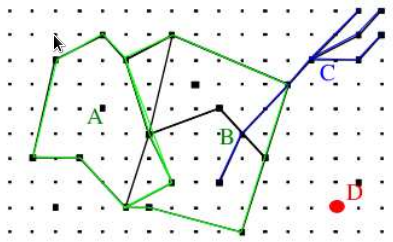
\includegraphics[scale=0.3]{Imagenes/4.png}\end{center}
\begin{small}
\end{small}
\end{frame}


\begin{frame}
\frametitle{Tipos de Datos y \'Algebras Espaciales}
Las b\'asicas abstracciones espaciales pueden ser embebidas en un DBMS existente usando tipos abstractos de datos.
\begin{itemize}
\item \textbf{Tipos de Datos Espaciales} encapsulan
\begin{small}
\begin{itemize}
\item la estructura de un objeto espacial, e.g., regi\'on
\item operaciones sobre esas estructuras
\end{itemize}
\end{small}
\item \textbf{\'Algebra Espacial}, es una colecci\'on de datos espaciales con operaciones relacionadas
\begin{itemize}
\begin{small}
\item Completitud y clausura deben ser propiedades del \'algebra
\end{small}
\end{itemize}
\end{itemize}
\end{frame}

\begin{frame}
\frametitle{\'Algebra ROSE}
\begin{variableblock}{ROSE (RObust Spatial Extension, G\"uting \& Schneider)}{bg=blue!50!white!70,fg=white}{bg=blue!50!black!70,fg=white}
\textit{Es un \'algebra espacial con tipos de datos espaciales basados en el modelo Realm (esto es, objetos compuestos por elementos realm)}
\end{variableblock}
\ \\
\textbf{Tipos de datos de ROSE}: puntos, l\'ineas y regiones.\\
\begin{center}
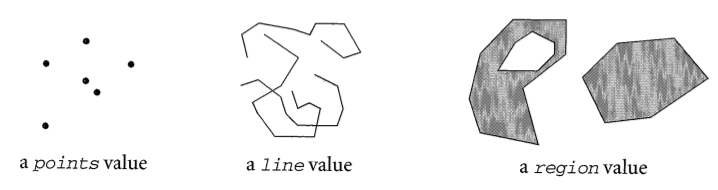
\includegraphics[scale=0.4]{Imagenes/5.png}
\end{center}
\end{frame}

\begin{frame}
\frametitle{\'Algebra ROSE: Operaciones}
EXT = $\lbrace$l\'ineas, regiones$\rbrace$\ \ \ \ GEO = $\lbrace$puntos, l\'ineas, regiones$\rbrace$\\
\ \\
\begin{itemize}
\item Predicados espaciales para relaciones topol\'ogicas:\\
\begin{itemize}
\item \textbf{inside}: geo $\times$ regions $\rightarrow$ bool
\item \textbf{intersect, meets}: ext1 $\times$ ext2 $\rightarrow$ bool
\item \textbf{adjacent, encloses}: regions $\times$ regions $\rightarrow$ bool
\end{itemize}
\item Operaciones que devuelven tipos de datos espaciales at\'omicos:\\
\begin{itemize}
\item \textbf{intersection}: lines $\times$ lines $\rightarrow$ points
\item \textbf{intersection}: regions $\times$ regions $\rightarrow$ regions
\item \textbf{plus, minus}: geo $\times$ geo $\rightarrow$ geo
\item \textbf{contour}: regions $\rightarrow$ lines
\end{itemize}
\end{itemize}
\end{frame}

\begin{frame}
\frametitle{\'Algebra ROSE: Operaciones}
EXT = $\lbrace$l\'ineas, regiones$\rbrace$\ \ \ \ GEO = $\lbrace$puntos, l\'ineas, regiones$\rbrace$\\
\ \\
\begin{itemize}
\item Operadores espaciales que devuelven n\'umeros:\\
\begin{itemize}
\item \textbf{dist}: geo1 $\times$ geo2 $\rightarrow$ real
\item \textbf{perimeter, area}: regions $\rightarrow$ real
\end{itemize}
\item Operadores espaciales en conjuntos de objetos:\\
\begin{itemize}
\item \textbf{sum}: set(obj) $\times$ (obj $\rightarrow$ geo) $\rightarrow$ geo
\item Alguna funci\'on espacial agregada como por ejemplo la suma de las \'areas de las provincias determinan el \'area de un pa\'is.
\item \textbf{closest}: set(obj) $\times$ (obj $\rightarrow$ geo1) $\times$ geo2 $\rightarrow$ set(obj)
\item Determina dentro de un conjunto de objetos aquellos cuyo atributo espacial tiene m\'inima distancia.
\item Otras operaciones complejas...
\end{itemize}
\end{itemize}
\end{frame}

\begin{frame}
\frametitle{\'Algebra ROSE: Propiedades}
Estos ejemplos son suficientes para ver qu\'e tipo de operaciones est\'an disponibles en un \'algebra espacial.\\
\ \\
Algunas propiedades que debe tener el \'algebra espacial son:\\
\begin{itemize}
\item Extensibilidad
\item Completitud
\item ?`Uno o m\'as tipos?
\item Operaciones de conjuntos
\end{itemize}
\end{frame}

\begin{frame}
\frametitle{Relaciones Espaciales}
Entre las operaciones espaciales, podemos distinguir las \textit{relaciones}.\\
\begin{itemize}
\item Topol\'ogicas: adjacent, inside, disjoint. Son invariantes dentro de transformaciones topol\'ogicas como scaling, rotation, translation.
\item De direcci\'on: above, below, north\_of.
\item M\'etricas: distance $<$ 100.
\end{itemize}
\ \\
Seis relaciones topol\'ogicas v\'alidas entre dos regiones simples (sin huecos, conectadas): disjoint, in, touch, equal, cover, overlap.
\end{frame}

\begin{frame}
\frametitle{Integrando la Geometr\'ia en el Modelo de Datos}
Los tipos de datos espaciales pueden ser embebidos en cualquier modelo de datos, e.g., el modelo relacional.\\
\ \\
El modelo de datos del DBMS debe ser extendido al nivel de tipos de datos at\'omicos, como strings y enteros.\\
\ \\
La idea b\'asica es representar \textbf{objetos espaciales} con objetos (del modelo de datos del DBMS) con al menos un atributo espacial.\\
\ \\
\begin{small}
Los objetos espaciales son tuplas con al menos un atributo espacial.\\
\texttt{\textbf{relation} estados (ename: STRING; area:REGION; epop: INTEGER)}\\
\texttt{\textbf{relation} ciudades (cname: STRING; centro:POINT; ext:REGION; cpop: INTEGER)}\\
\texttt{\textbf{relation} rios (rname: STRING; ruta:LINE)}\\
\end{small}
\end{frame}

\begin{frame}
\frametitle{Consultas}
Dos problemas principales:\\
\begin{itemize}
\item Conectar las operaciones del \'algebra espacial (incluyendo los predicados de relaciones espaciales) a las facilidades de un lenguaje de consulta de un DBMS.\\
Los operadores fundamentales son:
\begin{itemize}
\item Spatial selection
\item Spatial join
\item Overlay, fusion, ...
\end{itemize}
\item Proveer una representaci\'on gr\'afica de la informaci\'on espacial (o sea, los resultados de la consulta) y adem\'as una entrada gr\'afica para los valores en las consultas.
\end{itemize}
\end{frame}

\begin{frame}
\frametitle{Consultas: Selecci\'on Espacial}
\textbf{Selecci\'on Espacial}: retorna aquellos objetos que satisfacen un predicado espacial en la consulta.\\
\ \\
\begin{variableblock}{\textit{Todas las ciudades de Argentina}}{bg=blue!50!white!70,fg=white}{bg=blue!50!black!70,fg=white}
\texttt{SELECT cname FROM ciudades c \\
WHERE c.centro inside Argentina.area}
\end{variableblock}
\begin{variableblock}{\textit{Todas las grandes ciudades en un radio de 100km de Rosario}}{bg=blue!50!white!70,fg=white}{bg=blue!50!black!70,fg=white}
\texttt{SELECT cname FROM ciudades c \\
WHERE dist(c.centro, Rosario.centro) < 100\\
\ \ \ AND c.pop > 500k}
\end{variableblock}
\end{frame}

\begin{frame}
\frametitle{Consultas: Join Espacial}
\textbf{Join Espacial:} un join que compara cualesquiera dos objetos que fueron \textit{joineados} basado en un predicado que toma los valores espaciales de ambos.\\
\begin{variableblock}{\textit{Para cada r\'io de Argentina, encontrar todas las ciudades dentro de 50 kms}}{bg=blue!50!white!70,fg=white}{bg=blue!50!black!70,fg=white}
\texttt{SELECT r.rname, c.cname, length(intersection(r.ruta, c.area))\\
FROM rios r, ciudades c \\
WHERE r.ruta intersects Argentina.area \\
\ \ \ AND dist(r.ruta, c.area) < 50\\}
\end{variableblock} 

\end{frame}

\begin{frame}
\frametitle{Consultas: Otras operaciones}

\textbf{Overlay:} retorna las regiones que son el resultado de sobreposicionar dos particiones.\\
\ \\
\textbf{Fusion:} es una forma especial de agrupaci\'on. Para cada grupo obtenido, se forma la uni\'on de todos los valores de un atributo espacial.\\
\ \\
\textbf{Voronoi:} computa de una colecci\'on de objetos puntos \textit{S} la correspondiente colecci\'on de objetos regi\'on. Para cada punto \textit{p}, la regi\'on consiste de los puntos del plano m\'as cercanos a \textit{p}, y que no est\'en m\'as cercanos a otro punto de \textit{S}.  
\end{frame}


\begin{frame}
\frametitle{Consultas: I/O Gr\'afica}
?`C\'omo determinar \texttt{Argentina} en los ejemplos anteriores(input), o c\'omo mostrar \texttt{intersection(ruta,Argentina.area)} o \texttt{rio.ruta}(output)?\\
\ \\
Requerimientos para consultas espaciales:
\begin{itemize}
\item Tipos de datos espaciales.
\item Muestreo gr\'afico de los resultados de consulta.
\item Combinaci\'on gr\'afica de varios resultados de consultas.
\item Herramientas para interactuar con gr\'aficos de entrada y resultados.
\item Facilidad para verificar el contenido de una muestra.
\end{itemize}
\end{frame}


\begin{frame}
\frametitle{Formato de Datos Espaciales}
Existen dos est\'andares de representaci\'on:
\ \\
\begin{itemize}
\item \textbf{WKT} (Well Known Text)
\item \textbf{WKB} (Well Known Binary)
\end{itemize}
\end{frame}

\begin{frame}
\frametitle{Formato de Datos Espaciales: WKT}
Esta representaci\'on es una codificaci\'on en formato ASCII para describir objetos espaciales.\\
\ \\
Es usada por PostgreSQL en PostGIS, y tambi\'en en Google Maps.\\
\ \\
Podemos describir puntos, multipuntos, l\'ineas, pol\'igonos, multipol\'igonos, puntos en 3 dimensiones, etc\'etera.\\
\ \\
Sintaxis:\\
\begin{itemize}
\item Punto: \texttt{POINT(30 50)}
\item L\'inea: \texttt{LINESTRING(1 1, 5 5, 10 10)}
\item Pol\'igono: \texttt{POLYGON ( (0 0, 10 0, 10 10, 0 10, 0 0),(20 20, 20 40, 40 40, 40 20, 20 20))}
\end{itemize}
\end{frame}

\begin{frame}
\frametitle{Formato de Datos Espaciales: WKB}
WKB utiliza enteros sin signo de un byte, enteros sin signo de cuatro bytes, y n\'umeros de ocho bytes de doble precisi\'on (formato IEEE 754). Un byte son ocho bits.\\
\ \\
Por ejemplo, un valor WKB que corresponde a un \texttt{POINT(1 1)} consiste en esta secuencia de 21 bytes (cada uno representado aquí por dos d\'igitos hexadecimales):\\
\texttt{0101000000000000000000F03F000000000000F03F}\\
\ \\
\begin{tabular}{l l}
Orden de byte & 01 $\rightarrow$ LE o BE\\
Tipo WKB	  & 01000000 $\rightarrow$ tipo de objeto\\
X & 000000000000F03F\\
Y & 000000000000F03F\\
\end{tabular}\\
M\'as r\'apida que WKT, pero menos entendible para el usuario.
\end{frame}

\begin{frame}
\begin{center}
\textbf{INDEXACI\'ON ESPACIAL}
\end{center}
\end{frame}

\begin{frame}
\frametitle{Indexaci\'on Espacial}

Organiza el espacio y los objetos en \'el de forma tal que s\'olo son considerados la parte del espacio y los objetos que sean relevantes a una consulta.\\
\ \\
Es un mecanismo para decrementar el n\'umero de b\'usquedas.\\
\ \\
El objetivo es tratar de no visitar y tocar cada vez a todos los \textit{n} elementos en la BD.\\
\ \\
Los \'indices espaciales nos permiten optimizar la recuperaci\'on.\\

\end{frame}

\begin{frame}
\frametitle{Indexaci\'on Espacial}
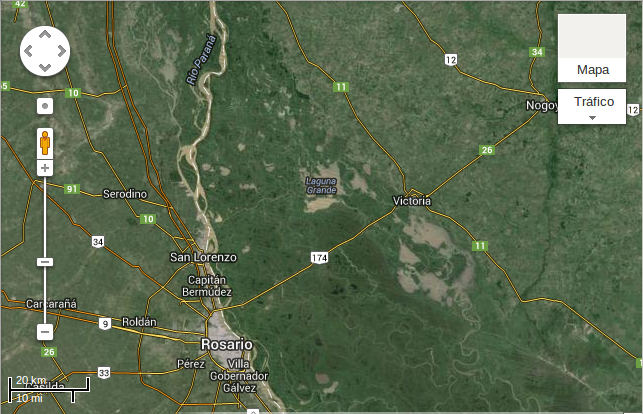
\includegraphics[scale=0.5]{Imagenes/6.png}
\end{frame}

\begin{frame}
\frametitle{Indexaci\'on Espacial}
El uso principal es para la selecci\'on espacial.\\
\begin{itemize}
\item Pero es usado tambi\'en para otras operaciones como join espacial o encontrar el objeto m\'as cercano...
\end{itemize}
Dos enfoques principales:
\begin{itemize}
\item Mapear objetos espaciales al espacio 1-D y utilizar t\'ecnicas est\'andar de indexaci\'on, como B-trees
\item Estructuras de indexaci\'on espacial dedicadas, como R-trees
\end{itemize}
\end{frame}

\begin{frame}
\frametitle{Indexaci\'on Espacial: R-Tree}
\textbf{R-Tree}\\
Es una estructura de datos similar a los B-Trees, con la diferencia que se utilizan para m\'etodos de acceso espacial. Es decir, podemos indexar coordenadas por ejemplo.\\
Cada nodo tiene un n\'umero variable de entradas, y cada entrada almacena dos datos: una forma de identificar a un nodo hijo y el conjunto l\'imite de todas las entradas de ese nodo hijo.\\
\textbf{B\'usqueda:} recursiva desde la ra\'iz, se verifica si el rect\'angulo de la consulta se solapa con alg\'un rect\'angulo del nodo.\\
\textbf{Inserci\'on:} partiendo de la ra\'iz, se usa una heur\'istica para seleccionar el nodo candidato.
\end{frame}

\begin{frame}
\frametitle{Indexaci\'on Espacial: R-Tree}
\textbf{R-Tree}\\
\begin{center}
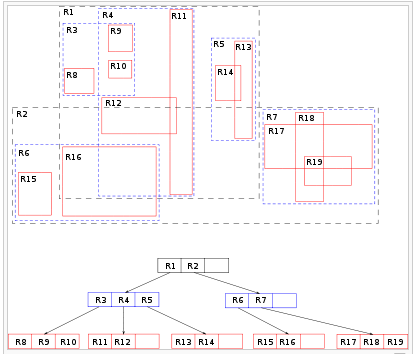
\includegraphics[scale=0.5]{Imagenes/20.png}
\end{center}
\end{frame}

\begin{frame}
\frametitle{Indexaci\'on Espacial}
La idea fundamental de la indexaci\'on espacial es la aproximaci\'on.\\
\begin{small}
\begin{itemize}
\item Aproximaci\'on continua
\item Aproximaci\'on por grilla
\end{itemize}
\end{small}
\begin{center}
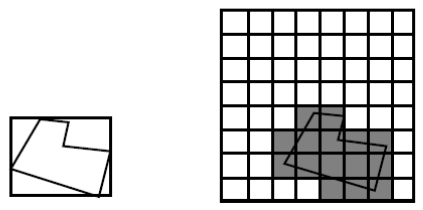
\includegraphics[scale=0.2]{Imagenes/7.png}
\end{center}
Para procesar una consulta, se procede a la estrategia de \textbf{filtrado y refinamiento}.
\begin{enumerate}
\item Filtrado: retorna un conjunto (donde est\'a la soluci\'on) de los valores posibles que satisfacen un predicado
\item Refinado: Para cada candidato, se refina la b\'usqueda chequeando la geometr\'ia
\end{enumerate}
\end{frame}

\begin{frame}
\frametitle{Indexaci\'on Espacial}
Las estructuras espaciales son dise\~nadas para almacenar puntos (para objetos puntos) o rect\'angulos (l\'ineas y regiones).\\
Las operaciones sobre esas estructuras son inserci\'on, borrado y pertenencia.\\
Consultas t\'ipicas:
\begin{itemize}
\item Puntos
\begin{itemize}
\item Consulta de rango: todos los puntos dentro de un rect\'angulo
\item Vecino m\'as cercano: el punto m\'as cercano a un punto consultado
\item Distancia: desde un punto, enumerar los puntos que est\'an a cierta distancia 
\end{itemize}
\item Rect\'angulos
\begin{itemize}
\item Intersecci\'on
\item Contenido
\end{itemize}
\end{itemize}
\end{frame}

\begin{frame}
\frametitle{Indexaci\'on Espacial: Estructuras}
\begin{itemize}
\item Una estructura de indexaci\'on espacial dedicada organiza los objetos en \textbf{cubetas}.
\item Cada cubeta tiene asociada una \textbf{regi\'on}, que es, una parte del espacio que contiene todos los objetos almacenados en esa cubeta.
\item Para estructuras de datos de puntos, las regiones son disjuntas
\begin{itemize}
\item el espacio es particionado y cada punto pertenece a solo una partici\'on (cubeta)
\begin{center}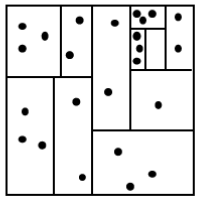
\includegraphics[scale=0.3]{Imagenes/8.png}
\end{center}\end{itemize}
\item Para estructuras con rect\'angulos, las cubetas pueden solaparse
\end{itemize}
\end{frame}

\begin{frame}
\frametitle{Indexaci\'on Espacial: Estructura de Puntos}
Estructuras espaciales para puntos: en $k$ dimensiones son representadas como una tupla $t = (x_1,...,x_k)$\\
\ \\
\textbf{\'Indice de Grilla}: Estructura de indexaci\'on espacial para puntos (Nievergelt, Hinterberger y Sevcik 84)
\begin{center}
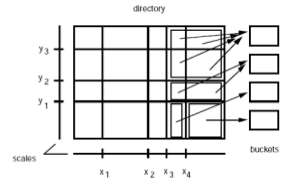
\includegraphics[scale=0.4]{Imagenes/9.png}
\end{center}
\begin{itemize}

\item El directorio es un arreglo $k$-dimensional cuyas entradas son punteros a las cubetas.
\item Todos los puntos en las celdas son almacenados en cubetas apuntando a la entrada de directorio correspondiente.
%\item Escalas peque\~nas. El directorio es almacenado en disco.
\end{itemize} 
\end{frame}

\begin{frame}
\frametitle{Indexaci\'on Espacial: Estructura de Puntos}
\textbf{kd-tree:}\\
\'Arbol binario donde cada nodo interno contiene un valor clave de una dimensi\'on.\\
La clave en el nodo ra\'iz (nivel 0) divide el espacio de datos con respecto a la dimensi\'on 0, las claves en sus hijos (nivel 1) divide los dos subespacios y as\'i sucesivamente hasta que se terminan las dimensiones, luego se reinicia el ciclo.\\
\begin{center}
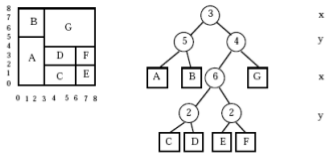
\includegraphics[scale=0.5]{Imagenes/10.png}
\end{center}
\end{frame}


\begin{frame}
\frametitle{Indexaci\'on Espacial: Estructura de Puntos}
\textbf{quad-tree:}\\
Divide el espacio de datos en forma recursiva en 4 cuadrantes (NO, NE, SO, SE)\\
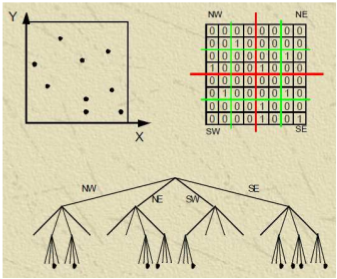
\includegraphics[scale=0.5]{Imagenes/11.png}
\end{frame}


\begin{frame}
\frametitle{Indexaci\'on Espacial: Estructura de Puntos}
\textbf{quad-tree:}\\
Hay diferentes algoritmos para procesar puntos, l\'ineas, pol\'igonos (i.e., distintos tipos de nodos, algoritmos de consultas).\\
Es usado muy frecuentemente en GIS comerciales para comprimir, almacenar y manipular im\'agenes raster.\\
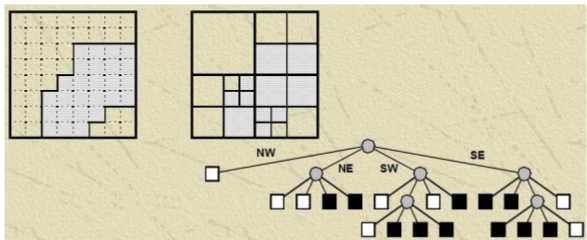
\includegraphics[scale=0.5]{Imagenes/12.png}
\end{frame}

\begin{frame}
\frametitle{Indexaci\'on Espacial: Estructura de Rect\'angulo}
Dos enfoques principales:
\begin{itemize}
\item Solapamiento de regiones
\item Clipping (Recorte)
\end{itemize}
\end{frame}

\begin{frame}
\frametitle{Indexaci\'on Espacial: Estructura de Rect\'angulo}
\textbf{Solapamiento de regiones}\\
Se abandona el espacio particionado y las regiones pueden solaparse, e.g., \textbf{R-tree}.\\
\begin{itemize}
\item Ventaja: El objeto espacial (clave) est\'a en una sola cubeta.
\item Desventaja: Muchos caminos terminan en un solapamiento de cubetas.
\end{itemize}
\begin{center}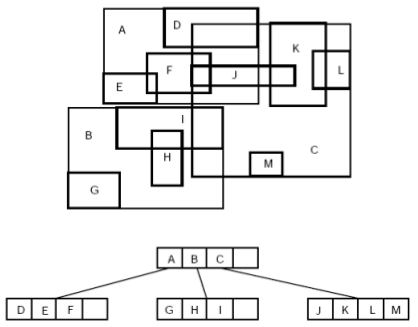
\includegraphics[scale=0.3]{Imagenes/13.png}
\end{center}
\end{frame}

\begin{frame}
\frametitle{Indexaci\'on Espacial: Estructura de Rect\'angulo}
\textbf{Recorte (Clipping)}\\
Las cubetas son disjuntas, pero los rect\'angulos son cortados en varias piezas, e.g., \textbf{R$^+$-tree}.\\
\begin{itemize}
\item Ventaja: Menos ramas en el \'arbol
\item Desventaja: M\'ultiples entradas para un objeto espacial
\end{itemize}
\begin{center}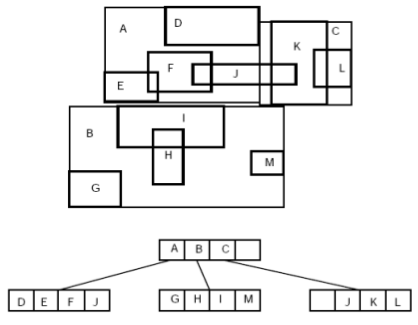
\includegraphics[scale=0.5]{Imagenes/14.png}
\end{center}
\end{frame}


\begin{frame}
\begin{center}
\textbf{ESTADO DEL ARTE}
\end{center}
\end{frame}

\begin{frame}

\frametitle{Spatial SQL}
?`C\'omo es Spatial SQL?\\
\ \\
Es igual que el SQL tradicional:
\begin{center}
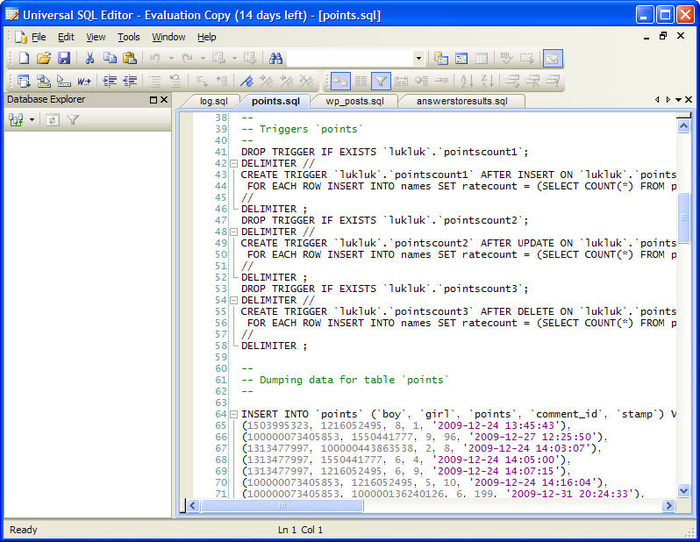
\includegraphics[scale=0.3]{Imagenes/21.png}
\end{center}
\end{frame}

\begin{frame}
\frametitle{Spatial SQL}
?`Es m\'as complicado?\\
\ \\
Puede, pero no tanto como SQL es:
\begin{center}
\begin{tiny}
\texttt{roadType,approachSpeed,recordID,Distance(Transform(GeomFromText(POINT(-1.5924443 54.7865551),4326),27700),PointN(Transform(geometry,27700),NumPoints(geometry)) ) AS DistanceToEnd,Distance(Transform(GeomFromText(POINT(-1.5924443 54.7865551),4326),27700),PointN(Transform(geometry,27700),1) ) AS DistanceFromStart,Distance(Transform(GeomFromText(POINT(-1.5924443 54.7865551),4326),27700),Transform(geometry,27700)) AS Distance FROM roads WHERE Distance(GeomFromText(POINT(-1.5924443 54.7865551),4326),geometry) < 0.0002 ORDER BY Distance(GeomFromText(POINT(-1.5924443 54.7865551),4326),geometry) LIMIT 1}
\end{tiny}
\end{center}
\end{frame}

\begin{frame}
\frametitle{Spatial SQL}
?`C\'omo es la informaci\'on espacial?\\
\ \\
\begin{center}
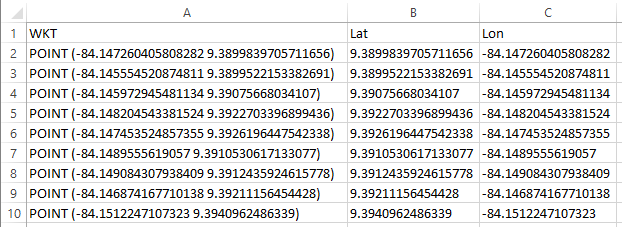
\includegraphics[scale=0.6]{Imagenes/22.png}
\end{center}
\end{frame}

\begin{frame}
\frametitle{Spatial SQL}
Nuevos tipos de datos
\begin{itemize}
\item Point
\item LineString
\item Polygon
\item MultiPoint
\item etc\'etera...
\end{itemize}

\end{frame}

\begin{frame}
\frametitle{Spatial SQL}
Relaciones
\begin{itemize}
\item ST\_Contains
\item ST\_Equals
\item ST\_Intersects
\item ST\_Touches
\item etc\'etera...
\end{itemize}

\end{frame}

\begin{frame}
\frametitle{Spatial SQL}
Constructores
\begin{itemize}
\item ST\_MultiLineString
\item ST\_Point
\item ST\_MultiPolygon
\item ST\_MultiCurve
\item etc\'etera...
\end{itemize}
\end{frame}

\begin{frame}
\frametitle{Spatial SQL: Ejemplo}
Crear una tabla nueva:\\
\ \\
\texttt{CREATE TABLE Rio(\\
\ \ \ \ \ Nombre varchar(30),\\
\ \ \ \ \ Origen varchar(30),\\
\ \ \ \ \ Longitud number,\\
\ \ \ \ \ Forma LineString );}
\end{frame}

\begin{frame}
\frametitle{Spatial SQL: Ejemplo}
\textbf{Consulta:} encontrar nombres de pa\'ises que son vecinos de Estados Unidos en la tabla Pa\'ises.\\
\ \\
\texttt{SELECT P1.Nombre\\
FROM Paises P1, Paises P2\\
WHERE Touch(P1.Forma,P2.Forma)=1\\
AND P2.Nombre = USA} 
\end{frame}

\begin{frame}
\frametitle{Spatial SQL: Ejemplo}
\textbf{Consulta:} encontrar la distancia entre dos puntos, dada una tabla de puntos.\\
\ \\
\texttt{SELECT ST\_Distance(geometrycolumn,\\
\ \ \ \ ST\_GeomFromText('POINT(1 2)',4326)\\
FROM tabladepuntos\\
ORDER BY\\
ST\_Distance(geometrycolumn,\\
\ \ \ \ ST\_GeomFromText('POINT(1 2)',4326) LIMIT 10)}
\end{frame}

\begin{frame}
\frametitle{Alternativas Espaciales}
Algunas de las elecciones que podemos hacer hoy en d\'ia en materia de DBMS espaciales son:\\
\textbf{Open Source}
\begin{itemize}
\item MySql (actualmente viene con soporte espacial)
\item MongoDB
\item MariaDB
\item PostgreSQL $+$ PostGIS
\item SpatialDB
\item y m\'as ...
\end{itemize}
\textbf{Pagos}
\begin{itemize}
\item Oracle
\item SQL Server
\end{itemize}

\end{frame}

\begin{frame}
\frametitle{PostgreSQL $+$ PostGIS}
\begin{center}
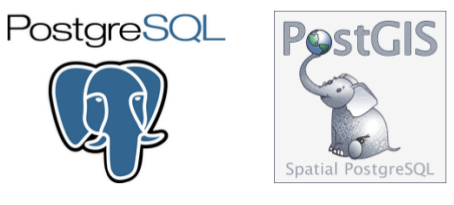
\includegraphics[scale=0.3]{Imagenes/23.png}
\end{center}
\begin{variableblock}{PostgreSQL}{bg=blue!50!white!70,fg=white}{bg=blue!50!black!70,fg=white}
\begin{itemize}
\item DBMS Open Source
\item Soporte para tablas de gran tama\~no y distintos tipos de datos
\end{itemize}
\end{variableblock}
\begin{variableblock}{PostGIS}{bg=blue!50!white!70,fg=white}{bg=blue!50!black!70,fg=white}
\begin{itemize}
\item Extensi\'on Espacial a PostgreSQL Open Source
\item Basado en las librer\'ias de C
\end{itemize}
\end{variableblock}
\end{frame}

\begin{frame}
\frametitle{PostgreSQL $+$ PostGIS}
\begin{variableblock}{Geometr\'ias B\'asicas}{bg=blue!50!white!70,fg=white}{bg=blue!50!black!70,fg=white}
\begin{itemize}
\item POINT 	(x y)
\item LINESTRING (x$_1$ y$_1$, ...,x$_n$ y$_n$)
\item POLYGON (x$_1$ y$_1$, ...,x$_n$ y$_n$)
\end{itemize}
\end{variableblock}
\begin{variableblock}{Multi-Geometr\'ias}{bg=blue!50!white!70,fg=white}{bg=blue!50!black!70,fg=white}
\begin{itemize}
\item MULTIPOINT ((POINT$_1$), ...,(POINT$_n$))
\item MULTILINESTRING ((LINESTRING$_1$), ...,(LINESTRING$_n$))
\item MULTIPOLYGON ((POLYGON$_1$), ...,(POLYGON$_n$))
\end{itemize}
\end{variableblock}
\end{frame}

\begin{frame}
\frametitle{PostgreSQL $+$ PostGIS}
Los constructores, operadores y relaciones son los que vienen con Spatial SQL, es decir, los mencionados anteriormente.\\
\ \\
\textit{PostGIS} agrega caracter\'isticas interesantes como su propio spatial join, GIS overlay functions, primitivas 2D y 3D, adem\'as de un entorno de desarrollo amigable.\\
\begin{center}
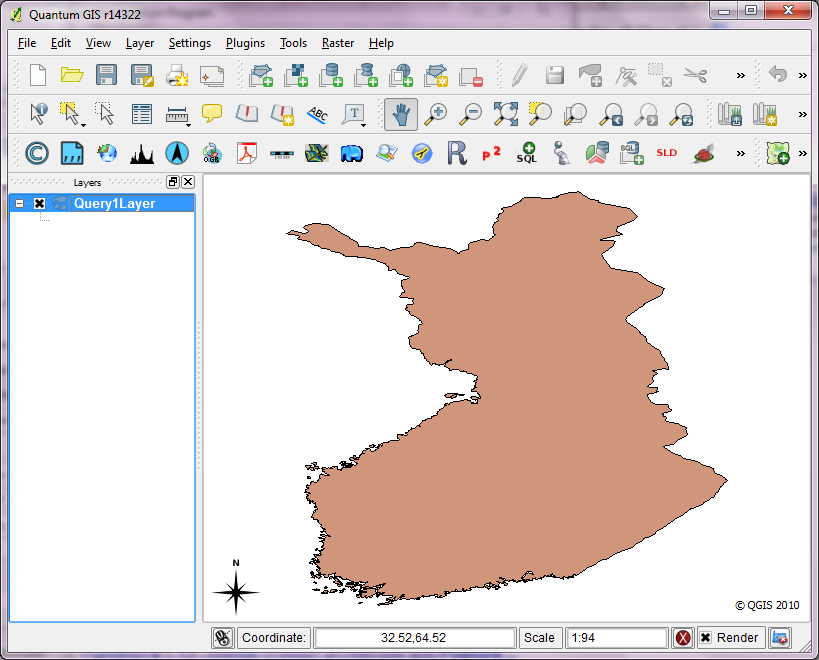
\includegraphics[scale=0.2]{Imagenes/24.png}
\end{center}
\end{frame}

\begin{frame}
\frametitle{Bibliograf\'ia}
\begin{itemize}
\item An Introduction to Spatial Database Systems, G\"uting. 
\item MySQL 5.7 Reference Manual.
\item Spatial Database Systems. Design,
Implementation and Project Management Series: GeoJournal Library, Yeung A., Hall K.W., Brent G.
\item T\'opicos Avanzados de Bases de Datos, Bender C. y Deco C.
\item PostGIS Documentation.
\end{itemize}
\end{frame}

\end{document}